\chapter{Perancangan}
Pada bab ini akan dijelaskan perancangan aplikasi pencarian rute terdekat
berbasis OpenStreetMap. Pada bagian pertama akan dijelaskan perancangan antar
muka untuk aplikasi yang akan dibangun. Diawali \textit{user} dengan membuka
aplikasi, selanjutnya \textit{user} dapat memilih titik-titik yang terdapat pada
peta sebagai titik asal ataupun titik tujuan. Setelah itu, \textit{user} dapat
mencari rute terdekat antara kedua titik tersebut.

Pada bagian kedua akan dijelaskan rancangan untuk aplikasi agar dapat
menjalankan fungsinya melalui diagram kelas. Pada bagian ketiga akan dijelaskan
bagaimana alur aplikasi dari \textit{user} hingga mengeluarkan \textit{output} yaitu rute terdekat
menggunakan diagram \textit{sequence}.

\section{Perancangan Antar Muka}
Pada subbab ini akan dijelaskan rancangan antar muka untuk aplikasi pencarian
rute terdekat. Aplikasi yang dibangun akan memiliki tampilan awal seperti pada
Gambar \ref{fig:mockup_1}.
\begin{figure}[h]
\centering
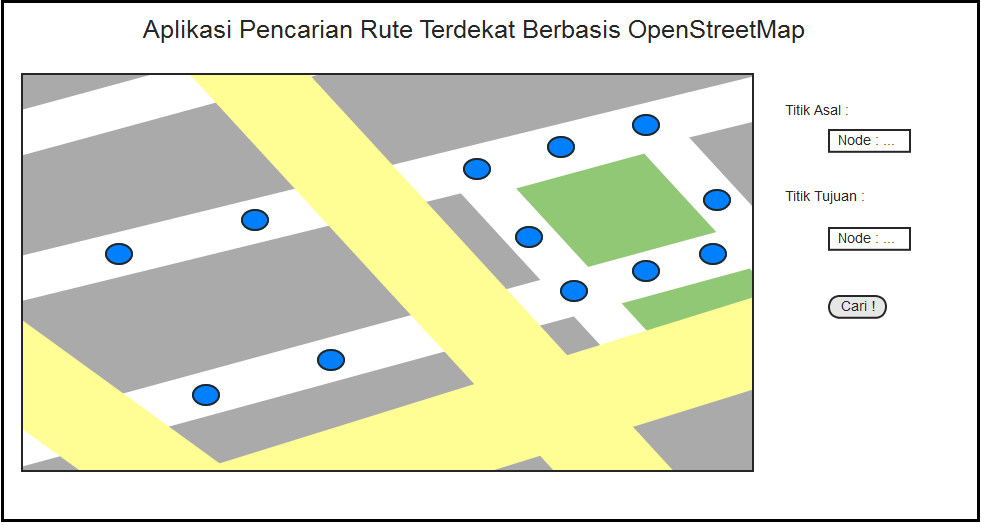
\includegraphics[scale=0.6]{Gambar/mockup_1}
\caption[Rancangan Antar Muka Awal Aplikasi]{Rancangan Antar Muka Awal Aplikasi}
\label{fig:mockup_1}
\end{figure}

Setelah halaman awal terbuka, \textit{User} dapat menekan setiap titik tersebut
dan akan menampilkan \textit{info window} yang memberikan informasi titik
beserta \textit{link}. \textit{User} dapat menekan \textit{link} tersebut untuk
menjadikannya sebagai titik asal ataupun titik tujuan. Rancangan antar muka saat
user memilih titik, dapat dilihat pada Gambar \ref{fig:mockup_2}.
\begin{figure}[h]
\centering
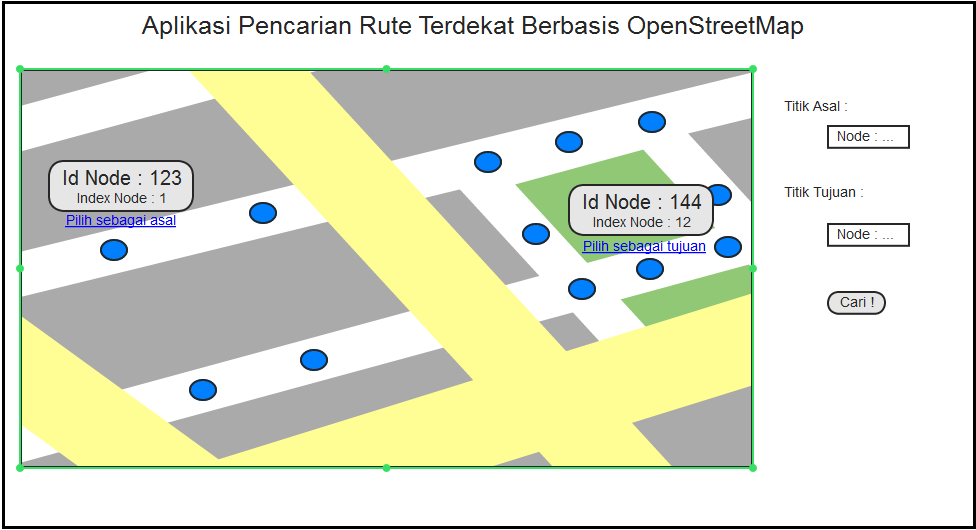
\includegraphics[scale=0.6]{Gambar/mockup_2}
\caption[Rancangan Pemilihan Titik]{Rancangan Pemilihan Titik}
\label{fig:mockup_2}
\end{figure}

Setelah user memilih titik asal dan titik tujuan, user dapat menekan tombol
``Cari!'' untuk melihat rute terdekat antara kedua titik tersebut. Rute tersebut
divisualisasikan dengan menggunakan \textit{polyline} yang berwarna merah.
Rancangan pada tahap ini dapat dilihat pada Gambar \ref{fig:mockup_3}.
\begin{figure}[h]
\centering
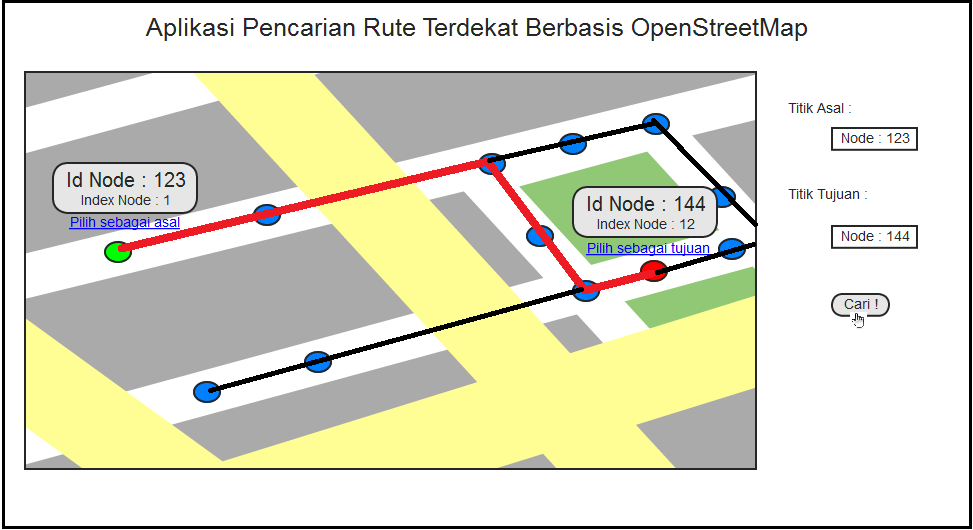
\includegraphics[scale=0.6]{Gambar/mockup_3}
\caption[Rancangan Cari Rute]{Rancangan Cari Rute}
\label{fig:mockup_3}
\end{figure}

\section{Perancangan Kelas}
Pada bagian ini akan dibahas perancangan kelas yang dilakukan untuk aplikasi
yang akan dibangun. Perancangan kelas bertujuan untuk menjelaskan
seluruh atribut dan fungsi yang akan diimplementasikan pada setiap kelas
yang sudah dibahas pada bab analisis. Perancangan kelas yang dibuat dapat 
dilihat pada Gambar \ref{fig:perancangan_kelas}. Berikut ini adalah penjelasan
dari setiap kelas beserta atribut dan fungsi yang digunakan:
\begin{itemize}
  \item Kelas XMLHttpRequest\\
  Kelas ini berfungsi untuk melakukan \textit{load} dokumen OSMXML.
  \begin{itemize}
    \item Fungsi
    \begin{itemize}
      \item open()\\
      Fungsi open() digunakan untuk membuka dokumen OSMXML.
      
      \item send()\\
      Fungsi send() digunakan untuk mengirimkan dokumen OSMXML yang sudah
      dibuka.
    \end{itemize}
  \end{itemize}
  
  \item Kelas Node dan Neighbor\\
  Kedua kelas ini akan menyimpan informasi yang didapatkan dari OSMXML sebagai
  representasi dari graf yaitu \textit{adjacency list}.
  \begin{itemize}
    \item Atribut Kelas Node
    \begin{itemize}
      \item id : int\\
      Atribut id menyimpan id node yang didapatkan dari dokumen OSMXML.
      
      \item adjList : Neighbor\\
      Atribut adjList menyimpan objek Neighbor.
    \end{itemize}
  \end{itemize}
  \begin{itemize}
    \item Atribut Kelas Neighbor
    \begin{itemize}
      \item vertexNum : int\\
      Atribut vertexNum menyimpan index dari node.
      
      \item next : Neighbor\\
      Atribut next menyimpan objek Neighbor.
      
      \item weight : double\\
      Atribut weight menyimpan jarak antar node.
    \end{itemize}
  \end{itemize}
  
  \item Kelas Graph\\
  Kelas ini berfungsi untuk mengubah informasi yang didapatkan dari OSMXML
  menjadi graf.
  \begin{itemize}
    \item Atribut
    \begin{itemize}
      \item adjLists : Array of Node\\
      Atribut adjLists merupakan \textit{array} yang menyimpan objek node.
      
      \item nd : Array\\
      Atribut nd menyimpan informasi berupa id node yang terdapat pada tag way
      di dalam dokumen OSMXML, atribut nd bertipe array.
      
      \item oneway : String\\
      Atribut nd menyimpan informasi berupa \textit{value} dari \textit{key}
      oneway yang terdapat pada tag way di dalam dokumen OSMXML, atribut oneway bertipe String.

\begin{figure}[h]
\centering
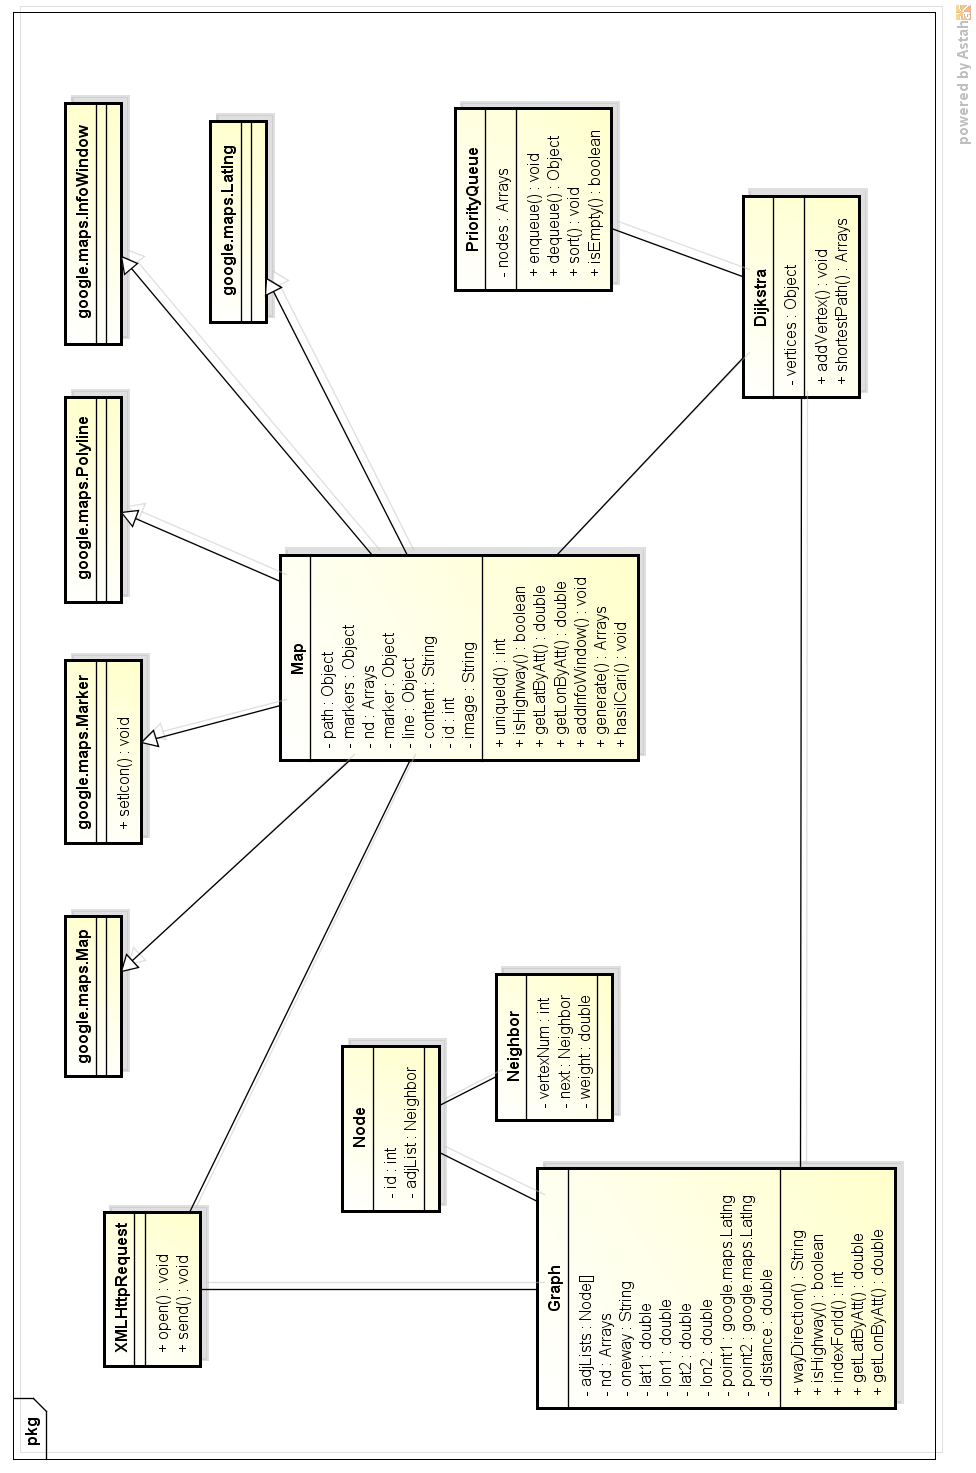
\includegraphics[scale=0.6]{Gambar/perancangan_kelas}
\caption[Diagram Kelas]{Diagram Kelas}
\label{fig:perancangan_kelas}
\end{figure}
\clearpage
    \end{itemize}
  \end{itemize}
  \begin{itemize}
    \item Fungsi
    \begin{itemize}
      \item wayDirection() : String\\
      Fungsi ini digunakan untuk mengetahui arah pada setiap node berdasarkan
      \textit{value} yang terdapat pada OSMXML.
      
      \item isHighway() : boolean\\
      Fungsi ini digunakan untuk melakukan \textit{filter} pada tag way, yaitu
      hanya way yang bertipe ``Highway'' saja yang akan digunakan pada pemodelan
      graf.
      
      \item indexForId() : int\\
      Fungsi ini digunakan untuk mengetahui index node pada graf berdasarkan id
      node.
      
      \item getLatByAtt() : double\\
      Fungsi ini digunakan untuk mendapatkan informasi \textit{latitude} pada
      sebuah node berdasarkan atributnya, yaitu id node.
      
      \item getLonByAtt() : double\\
      Fungsi ini digunakan untuk mendapatkan informasi \textit{longitude} pada
      sebuah node berdasarkan atributnya, yaitu id node.
    \end{itemize}
  \end{itemize}
  
  \item Kelas Map\\
  Kelas ini berfungsi untuk melakukan \textit{generate} peta, visualisasi graf,
  dan visualisasi rute terdekat.
  \begin{itemize}
    \item Atribut
    \begin{itemize}
      \item path : Object\\
      Atribut path adalah variabel yang menyimpan informasi titik koordinat
      dalam bentuk objek, atribut path digunakan untuk pembuatan \textit{marker}
      dan \textit{polyline}.
      
      \item markers : Object\\
      Atribut ini menyimpan seluruh objek \textit{marker}.
      
      \item nd : Arrays\\
      Atribut nd menyimpan informasi berupa id node yang terdapat pada tag way
      di dalam dokumen OSMXML, atribut nd bertipe array.
      
      \item marker : Object\\
      Atribut ini menyimpan objek \textit{marker} untuk ditampilkan pada peta.
      
      \item line : Object\\
      Atribut ini menyimpan objek \textit{polyline} untuk ditampilkan pada peta.
      
      \item content : String\\
      Atribut ini merupakan isi dari \textit{info window} yang disisipkan pada
      setiap marker. Atribut ini berisi id node, index node, \textit{link} titik
      asal, dan \textit{link} titik tujuan.
      
      \item id : int\\
      Atribut ini merupakan id yang digunakan untuk melakukan \textit{generate}
      id pada fungsi uniqueId. 
      
      \item image : String\\
      Atribut ini menyimpan alamat dari \textit{image} atau gambar yang
      digunakan oleh \textit{marker}.
    \end{itemize}
  \end{itemize}
  \begin{itemize}
    \item Fungsi
    \begin{itemize}
      \item uniqueId() : id\\
      Fungsi ini digunakan untuk melakukan \textit{generate} id, id tersebut
      digunakan oleh \textit{marker}.
      
      \item isHighway() : boolean\\
      Fungsi ini digunakan untuk melakukan \textit{filter} pada tag way, hanya
      way yang bertipe ``Highway'' saja yang digunakan. Fungsi ini digunakan
      pada saat pembuatan objek \textit{marker} pada peta.
      
       \item getLatByAtt() : double\\
      Fungsi ini digunakan untuk mendapatkan informasi \textit{latitude} pada
      sebuah node berdasarkan atributnya, yaitu id node.
      
      \item getLonByAtt() : double\\
      Fungsi ini digunakan untuk mendapatkan informasi \textit{longitude} pada
      sebuah node berdasarkan atributnya, yaitu id node.
      
      \item addInfoWindow()\\
      Fungsi ini digunakan untuk menambahkan objek \textit{info window} pada
      setiap \textit{marker}.
      
      \item generate() : Arrays\\
      Fungsi ini digunakan untuk menampilkan secara keseluruhan \textit{marker}
      dan \textit{polyline} pada peta. Fungsi akan mengembalikan
      objek \textit{marker} di dalam bentuk array.
      
      \item hasilCari()\\
      Fungsi ini digunakan untuk melakukan visualisasi rute terdekat menggunakan
      \textit{polyline}.
    \end{itemize}
  \end{itemize}
  
  \item Kelas google.maps.Map\\
  Kelas ini berfungsi untuk membuat objek peta.
  
  \item Kelas google.maps.Marker\\
  Kelas ini berfungsi untuk membuat objek \textit{marker} yang akan digunakan
  sebagai visualisasi node pada peta.
  \begin{itemize}
    \item Fungsi
    \begin{itemize}
      \item SetIcon()\\
      Fungsi ini digunakan untuk mengubah icon dari \textit{marker}.
    \end{itemize}
  \end{itemize}
  
  \item Kelas google.maps.Polyline\\
  Kelas ini berfungsi untuk membuat objek \textit{polyline} yang akan digunakan
  sebagai visualisasi edge pada peta.
  
  \item Kelas google.maps.InfoWindow\\
  Kelas ini berfungsi untuk membuat objek \textit{InfoWindow} yang akan
  disisipkan pada setiap objek \textit{marker}.
  
  \item Kelas google.maps.Latlng\\
  Kelas ini berfungsi untuk membuat objek Latlng. Latlng merupakan objek yang
  berisi informasi koordinat (\textit{latitude} dan \textit{longitude}).
  
  \item Kelas Dijkstra\\
  Kelas ini berfungsi untuk mencari rute terdekat berdasarkan \textit{input}
  titik asal dan titik tujuan.
  \begin{itemize}
    \item Atribut
    \begin{itemize}
      \item nodes : Object\\
      Atribut ini menyimpan informasi node dalam bentuk objek.
    \end{itemize}
  \end{itemize}
  \begin{itemize}
    \item Fungsi
    \begin{itemize}
      \item addNode()\\
      Fungsi ini digunakan untuk menambahkan satu node beserta edgenya.
      
      \item shortestPath() : Arrays\\
      Fungsi ini digunakan untuk pencarian rute terdekat, fungsi akan
      mengembalikan rute atau jalur terpendek dalam bentuk array.
    \end{itemize}
  \end{itemize}
  
  \item Kelas PriorityQueue\\
  Kelas ini merupakan struktur data \textit{queue} yang digunakan pada
  kelas dijkstra.
  \begin{itemize}
    \item Atribut
    \begin{itemize}
      \item queue : Array\\
      Atribut ini merupakan \textit{queue} dari kelas PriorityQueue.
    \end{itemize}
  \end{itemize}
  \begin{itemize}
    \item Fungsi
    \begin{itemize}
      \item enqueue()\\
      Fungsi ini digunakan untuk menambahkan objek ke dalam \textit{queue}.
      
      \item dequeue() : Object\\
      Fungsi ini digunakan untuk mengeluarkan objek dari dalam \textit{queue}.
      
      \item sort()\\
      Fungsi ini digunakan untuk menyusun \textit{queue}.
      
      \item isEmpty() : boolean\\
      Fungsi ini digunakan untuk pengecekan isi dari \textit{queue}. jika
      \textit{queue} kosong, fungsi akan mengembalikan ``true'' dan sebaliknya
      ``false'' jika \textit{queue} tidak kosong.
    \end{itemize}
  \end{itemize}
\end{itemize}

\section{Diagram Sekuens}
Diagram sekuens adalah diagram yang digunakan untuk menggambarkan interaksi
antara objek dengan waktu, interaksi tersebut digambarkan dengan grafik dua
dimensi. Kedua dimensi tersebut adalah dimensi horizontal dan dimensi vertikal.
Dimensi horizontal menggambarkan objek-objek yang berperan, sedangkan dimensi
vertikal menggambarkan waktu. Pesan yang dikirimkan oleh suatu objek digambarkan
dengan panah dan panah dengan garis putus-putus menggambarkan pesan balasan.
Diagram sekuens pada bagian ini mengacu kepada diagram \textit{use case} yang
terdapat pada bab 3, dapat dilihat pada Gambar \ref{fig:usecase}. Berikut ini
adalah diagram sekuens berdasarkan diagram \textit{use case} tersebut:
\begin{enumerate}
  \item Pemilihan Titik Asal\\
  Diagram sekuens untuk pemilihan titik asal dapat dilihat pada Gambar
  \ref{fig:sd_titikAsal}.
\begin{figure}[h]
\centering
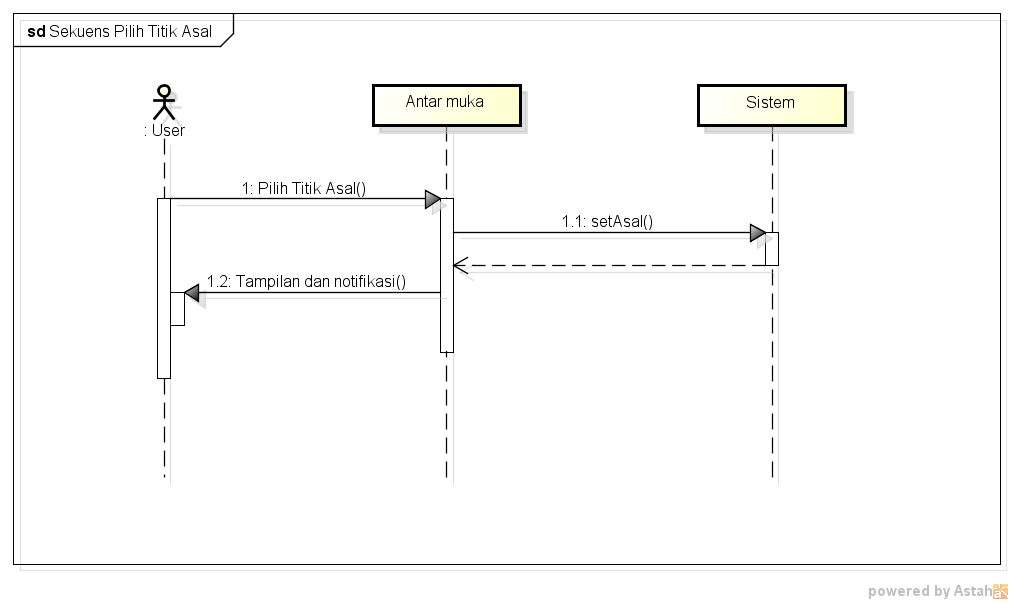
\includegraphics[scale=0.5]{Gambar/sd_titikAsal}
\caption[Diagram Sekuens Pemilihan Titik Asal]{Diagram Sekuens Pemilihan Titik
Asal}
\label{fig:sd_titikAsal}
\end{figure}
  
  \item Pemilihan Titik Tujuan\\
  Diagram sekuens untuk pemilihan titik asal dapat dilihat pada Gambar
  \ref{fig:sd_titikTujuan}.
\begin{figure}[h]
\centering
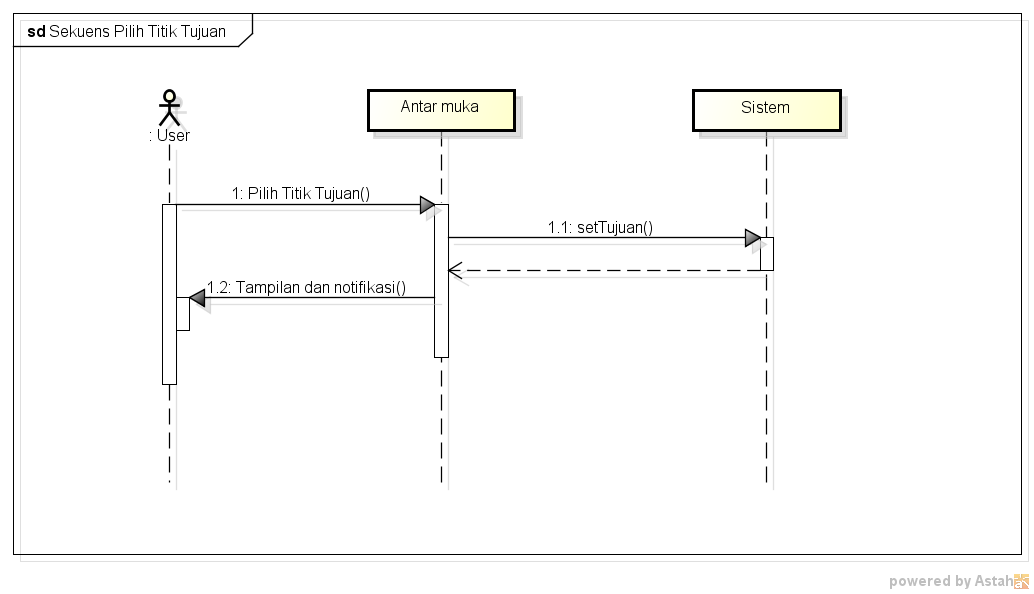
\includegraphics[scale=0.5]{Gambar/sd_titikTujuan}
\caption[Diagram Sekuens Pemilihan Titik Tujuan]{Diagram Sekuens Pemilihan Titik
Tujuan}
\label{fig:sd_titikTujuan}
\end{figure}
  
  \item Pencarian Rute Terdekat\\
  Diagram sekuens untuk pencarian rute terdekat dapat dilihat pada Gambar
  \ref{fig:sd_rute}.
\begin{figure}[h]
\centering
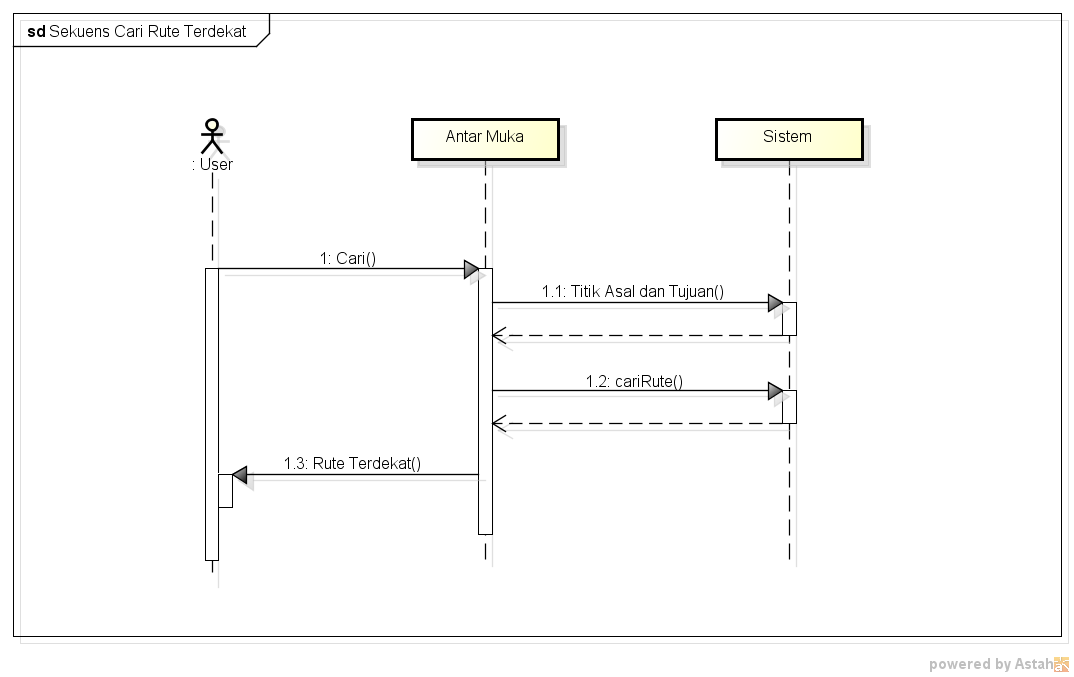
\includegraphics[scale=0.5]{Gambar/sd_rute}
\caption[Diagram Sekuens Pencarian Rute Terdekat]{Diagram Sekuens Pencarian Rute Terdekat}
\label{fig:sd_rute}
\end{figure}
\end{enumerate}